\documentclass[11pt,a4paper]{article}

% Required packages
\usepackage[utf8]{inputenc}
\usepackage[T1]{fontenc}
\usepackage{times} % Times New Roman font
\usepackage{CJK} % For Japanese text support
\usepackage{geometry}
\usepackage{multicol}
\usepackage{setspace}
\usepackage{graphicx}
\usepackage{xcolor}
\usepackage{fancyhdr}
\usepackage{titlesec}
\usepackage{caption}     % For \captionof

% Page geometry setup
\geometry{
    a4paper,
    top=25mm,
    bottom=30mm,
    left=18mm,
    right=18mm
}

% Remove page numbers
\pagestyle{empty}

% Configure two-column layout
% Column width: 83.5mm each, spacing: 7mm
\setlength{\columnsep}{7mm}
\setlength{\columnwidth}{83.5mm}

% Configure section titles (chapter titles)
\titleformat{\section}
{\normalfont\fontsize{11}{13}\bfseries}{\thesection}{1em}{}

\titleformat{\subsection}
{\normalfont\fontsize{11}{13}\bfseries}{\thesubsection}{1em}{}

% Line spacing to achieve approximately 60 lines per column
\linespread{1.0}

% Remove paragraph indentation and add spacing
\setlength{\parindent}{0pt}
\setlength{\parskip}{0.5ex}

\begin{document}

% First page header setup (6 lines from top)
\begin{center}
% Line 1: blank
~\\
% Line 2: Title in English (Times New Roman, 12pt, Center)
{\fontsize{12}{14}\selectfont \textbf{A Multifaceted Exploration of Spatial Openness in Rental Housing: Big Data Analysis Across Tokyo's 23 Wards}}\\
% Line 3: Title in Japanese (MS Mincho, 11pt, Center)
\begin{CJK}{UTF8}{min}
{\fontsize{11}{13}\selectfont 賃貸住宅における空間開放性の多面的探究:東京23区のビッグデータ分析}
\end{CJK}\\
% Line 4: blank
~\\
\end{center}

% Line 5: Affiliation, Student ID, Name (Times New Roman, 11pt, Right-justified)
\begin{flushright}
{\fontsize{11}{13}\selectfont Oki Lab , Student ID: 23M5833, Yuan Liu}
\end{flushright}

% Line 6: blank
~\\

% Main body starts from line 7
\begin{multicols}{2}
\fontsize{11}{13}\selectfont

\section{Introduction}

Spatial openness is a critical factor in property selection and residential design, encompassing
perceived spaciousness, visual connectivity, and flow within living environments. Understanding
and quantifying spatial openness is essential for real estate professionals and architectural
designers seeking to optimize residential spaces.

Traditional approaches to analyzing spatial openness rely on structured data analysis using
standardized metrics such as floor area, room count, and basic dimensional measurements. These
conventional methods fail to capture the nuanced spatial qualities that truly define openness
and rarely leverage rich, unstructured data sources such as interior imagery and floor plan
(madori) data.

This research proposes a novel methodology that harnesses innovative information sources through
advanced computational techniques. Our approach integrates interior images with semantic
segmentation, floor plan images processed through semantic segmentation, and optical image-based
visibility graph analysis (VGA). This methodology breaks traditional VGA constraints that
historically required manual data inputs such as AutoCAD vectorized maps and proprietary
software like DepthMapX.

Our method utilizes open-source coding frameworks that significantly accelerate data processing
capabilities, enabling analysis of substantially larger datasets. By reducing manual processes
required by traditional spatial analysis tools, our approach enables fully automated processing
pipelines for large-scale datasets, opening new possibilities for comprehensive urban-scale
studies of residential spatial quality.

\section{Data Source and Preprocessing}

The data source for this study is the rental category of data from the Lifull dataset. In this study, 
we focus on the rental property in Tokyo area, constructed date from 1960 to most recent years. Every 
decades we sampled roughly 1000 to 1500 properties to make the distribution more balanced. Since we 
need clear interior images for interior semseg analysis, clear madori images to extract the VGA distributions,
and compare the properties visual elements from those images to their tabular specs data, we have to screen 
outs those poor quality images and very incomplete infos, after the filtering we have around 6000 
properties left. As illustrated in Figure \ref{fig:samplesize_decades}, our dataset demonstrates a comprehensive coverage 
across Tokyo's 23 wards spanning multiple construction decades. 
% Image inside multicols environment to fit within one column
% \begin{figure}[htbp]
\begin{center}
    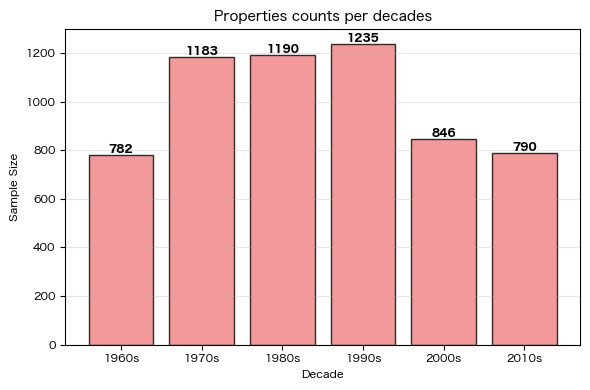
\includegraphics[width=\columnwidth]{plots/samplesize_decades.png}
    \captionof{figure}{Dataset overview showing property construction date distribution across Tokyo's 23 wards.}
    \label{fig:samplesize_decades}
\end{center}
% \end{figure}

The entire data processing pipeline remains stable and fast in this level, the whole 
processing time can be finished within a couple of hours, though depends on the actual specs of the 
machine. We will mention about the details in the thesis when it comes to the actual technical steps.



\section{Quantifying the Openness of Residential Spaces}

We focus on several key quantifiable statistics that might be related to the openness of properties, beyond the 
already existing tabular features such as room types and room area.

From interior data, we first filtered the main living room images, then applied semantic segmentation using the 
Mask2Former model which is pretrained on the ADE20K dataset to ensure that key components such as walls, ceilings, 
and windows can be correctly tagged. We then extract the ratio of their appearance in each image as features for 
later analysis, as shown in Figure \ref{fig:interior_semseg}. 
\begin{flushleft}
    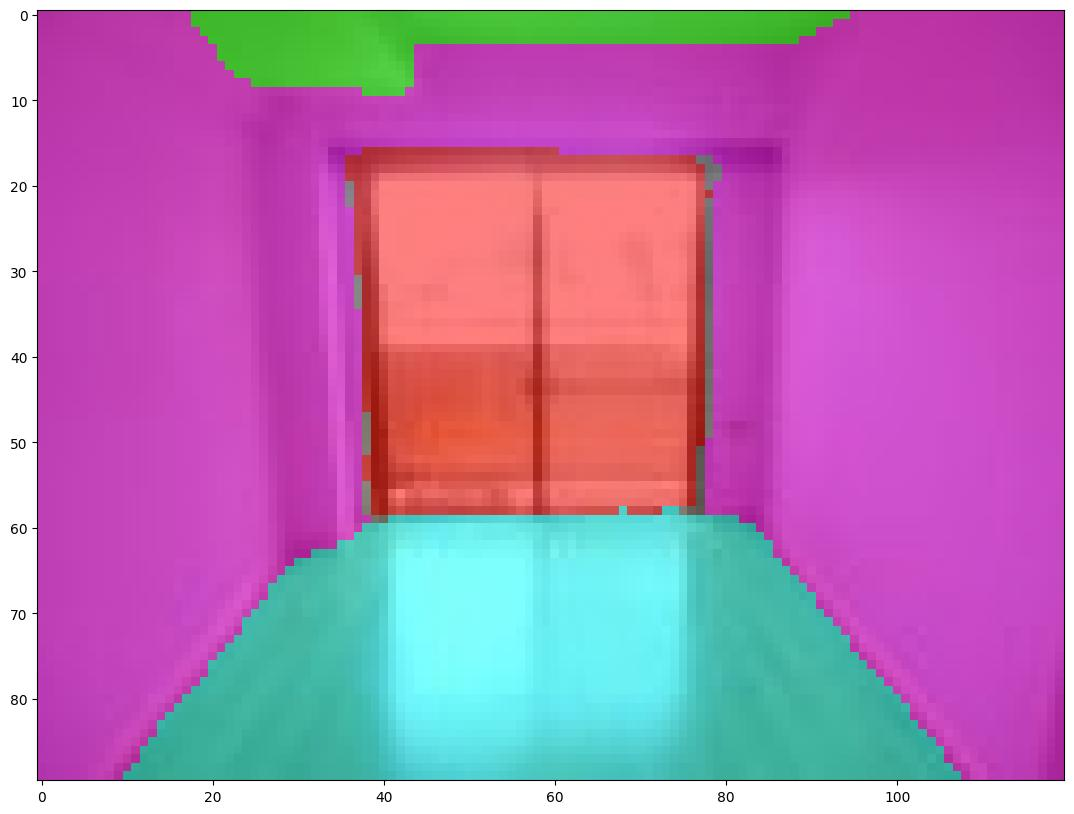
\includegraphics[width=0.8\columnwidth]{plots/exp_lv_semseg_2.jpg}
    \\[0.5em]
    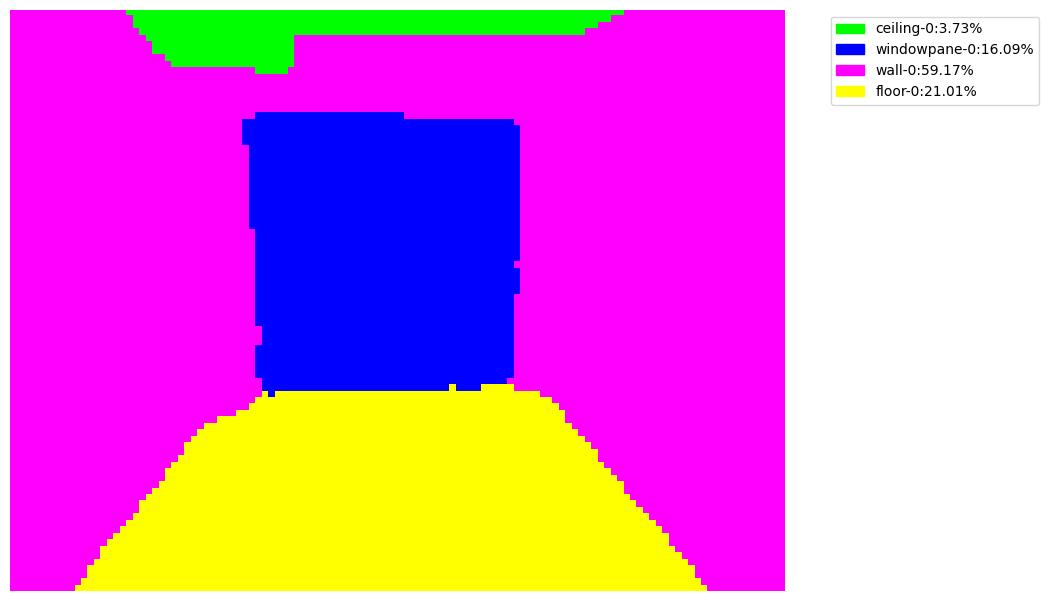
\includegraphics[width=\columnwidth]{plots/exp_lv_semseg_1.jpg}
    \captionof{figure}{Example of interior semantic segmentation results.}
    \label{fig:interior_semseg}
\end{flushleft}


From madori (floorplan) data, we first performed semantic segmentation using a model pretrained on non-floorplan 
data, then utilized a labeled dataset to perform fine-tuning to ensure it can classify floorplan components like 
walls, bedrooms, living rooms, etc. 
\begin{flushleft}
    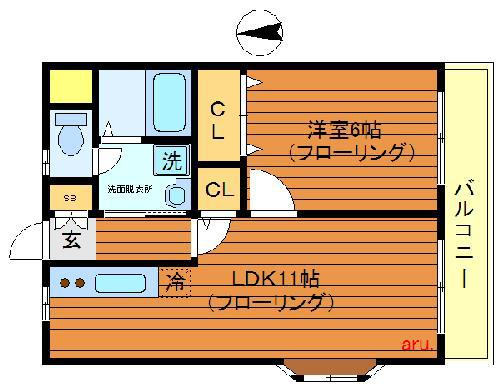
\includegraphics[width=0.7\columnwidth]{plots/exp_maodri_semseg_raw.jpg}
    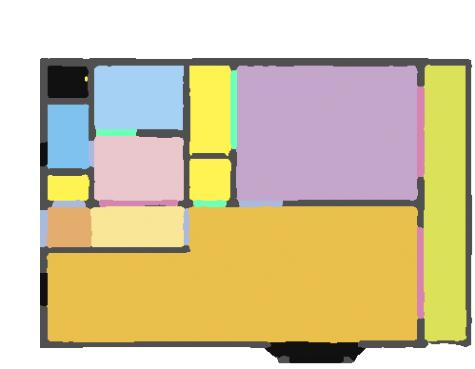
\includegraphics[width=0.7\columnwidth]{plots/exp_madori_semseg_decoded.jpg}
    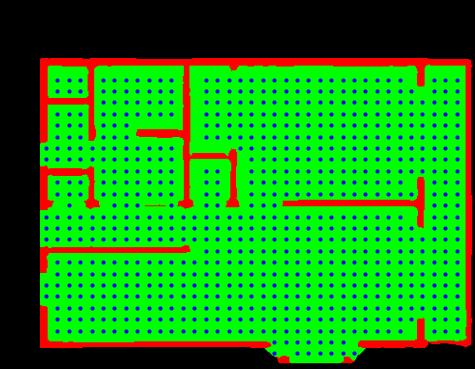
\includegraphics[width=0.7\columnwidth]{plots/exp_madori_semseg_grid.jpg}
    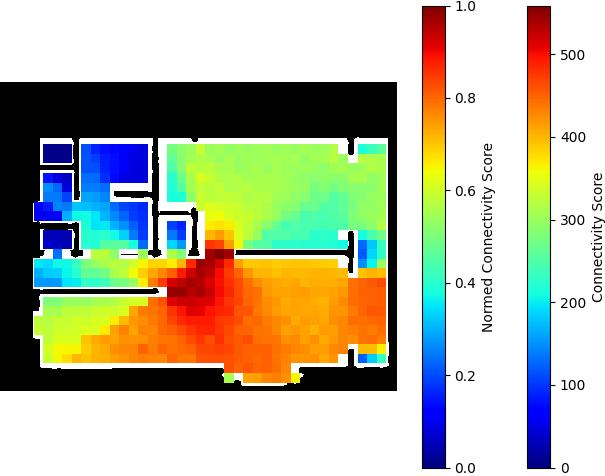
\includegraphics[width=0.7\columnwidth]{plots/exp_madori_semseg_vga.jpg}
    \captionof{figure}{From top to bottom: raw floorplan, the semantic segmentation output, the physical gridding, and the heatmap of VGA.}
    \label{fig:madori_processing}
\end{flushleft}

To obtain VGA scores, we extract the open area by filtering out the background 
and walls. Then, by a given granularity, we create a grid over the area. Since every property has different 
physical dimensions, we normalize the density of gridding by physical size, with each grid cell ranging around 20~cm.

We define the VGA value at each grid node by the number of visible nodes from that node:
\begin{equation}
\label{eq:vga_definition}
S(i) = \sum_{j=1}^{N} V_{ij}
\end{equation}
where $S(i)$ is the visibility score at node $i$, $N$ is the total number of nodes, and $V_{ij} = 1$ if node $j$ 
is visible from node $i$, otherwise $V_{ij} = 0$.
By this method, a VGA heatmap can be generated, and we extract VGA scores by taking the mean, standard deviation, 
minimum/maximum, etc., over the whole property or only living rooms to represent its VGA features. 
The output result with the raw floorplan input for the above processings are demonstrated in the following graph 
as shown in Figure \ref{fig:madori_processing}.

% \fontsize{11}{13}\selectfont

\section{Influence of building age and geographic factors.}
From the tabular features of the properties, we have various information, with the most interesting being building age and geographic factors. 
We examined the distribution of VGA mean values across construction dates in decades, as shown in Figure \ref{fig:vga_10years_box}.
Similarly, we examined the distribution of q3 impression scores across construction dates in decades, as shown in Figure \ref{fig:q3_10years_box}.

\begin{flushleft}
    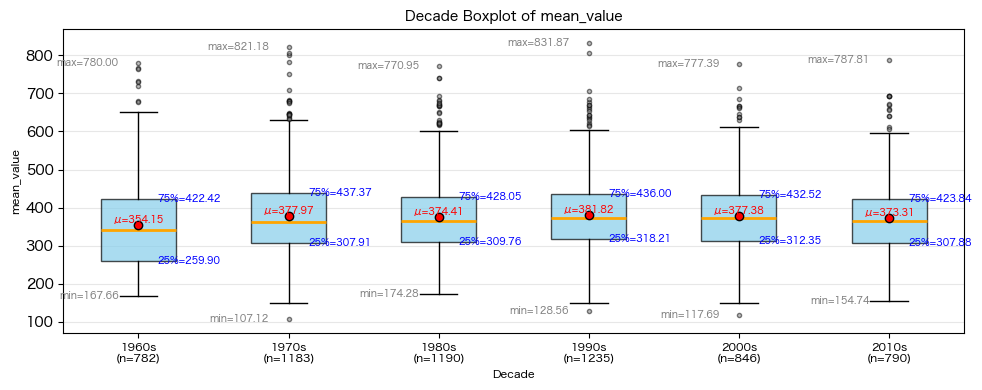
\includegraphics[width=0.9\columnwidth]{plots/vga_10years_box.png}
    \captionof{figure}{Distribution of VGA mean values across construction dates by decade}
    \label{fig:vga_10years_box}
\end{flushleft}
\begin{flushleft}
    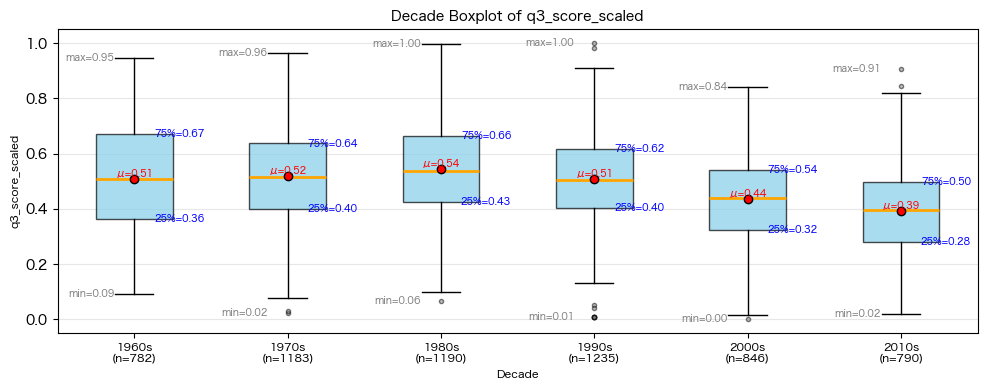
\includegraphics[width=0.9\columnwidth]{plots/q3_10years_box.png}
    \captionof{figure}{Distribution of q3 impression scores by property construction decade}
    \label{fig:q3_10years_box}
\end{flushleft}

From the distribution analysis, we observe that VGA mean values, which are heavily influenced by floorplan layout and property size, 
contain more large outliers while remaining relatively stable across decades. This pattern potentially reflects the impact of large-area properties 
on the overall distribution. Meanwhile, the q3 impression scores show a more balanced distribution, 
which is reasonable since impression scores evaluated from single interior photographs are more independent of the entire property layouts.

Figure \ref{fig:tokyo23_exp} presents VGA analysis results and q3 impression score distributions across Tokyo's 23 special wards. 
The visualization demonstrates regional variations in spatial openness characteristics, 
providing insights into urban housing design patterns 
at the metropolitan scale.
\begin{flushleft}
    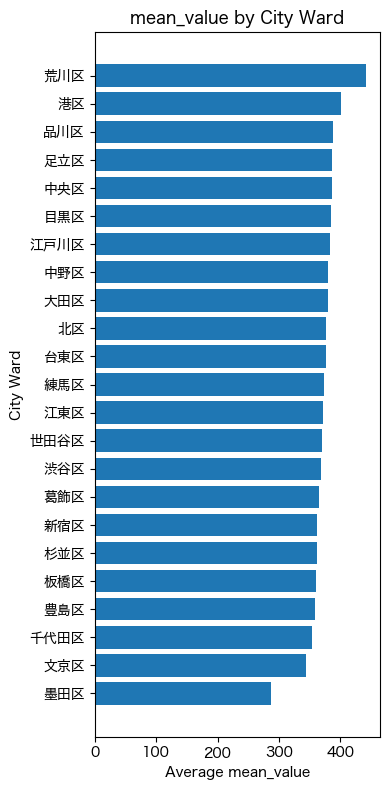
\includegraphics[width=0.45\columnwidth]{plots/tokyo23_vga.png}
    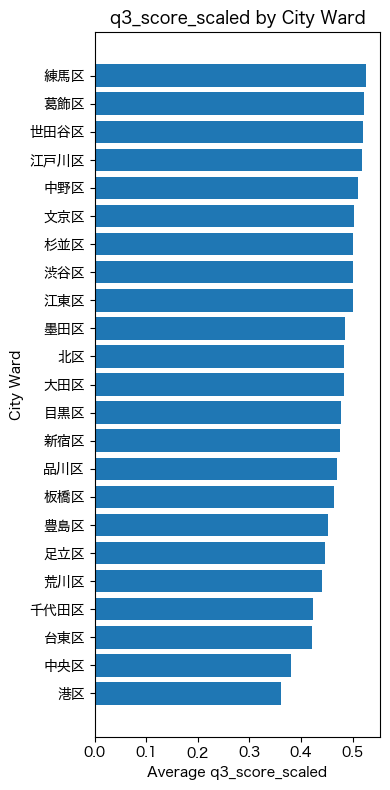
\includegraphics[width=0.45\columnwidth]{plots/tokyo23_q3.png}
    \captionof{figure}{VGA mean values and q3 impression score distributions across Tokyo's 23 special wards}
    \label{fig:tokyo23_exp}
\end{flushleft}




% \fontsize{11}{13}\selectfont
\section{Correlation Analysis Between Subjective Impressions and Openness}

To validate our approach, we analyzed correlations between computed spatial metrics and subjective impressions 
using a pre-trained model by Shimomura et al. that outputs impression scores (q3) from interior images.
We extracted VGA statistics from floorplans overlaid with living room masks to match the q3 model's training data scope.
However, no significant correlation was found between VGA metrics and q3 scores, as shown in Figure \ref{fig:corr_vga_q3}.
This stems from a fundamental mismatch: q3 uses limited-view interior photographs while VGA analyzes complete floorplan layouts.

We also examined correlations between interior semantic segmentation component ratios and q3 scores. 
After filtering outliers using centered clustering with a 75th percentile cutoff, the results are shown 
in Figures \ref{fig:inter_q3_cluster} and \ref{fig:corr_inter_q3}.

Interior segmentation analysis shows window and wall components have very weak correlation with impression scores, 
while floor and ceiling exhibit mild to moderate negative correlations. This suggests excessive floor or ceiling 
visibility negatively impacts quality perceptions, emphasizing the importance of balanced camera angles.

We also analyzed correlations between VGA statistics, interior segmentation results, and property data.
Figure \ref{fig:q3_10years_box} shows q3 impression scores by construction decade, revealing trends in 
perceived spatial quality over time. This demonstrates how our framework can identify temporal patterns 
in housing design preferences.
\begin{flushleft}
    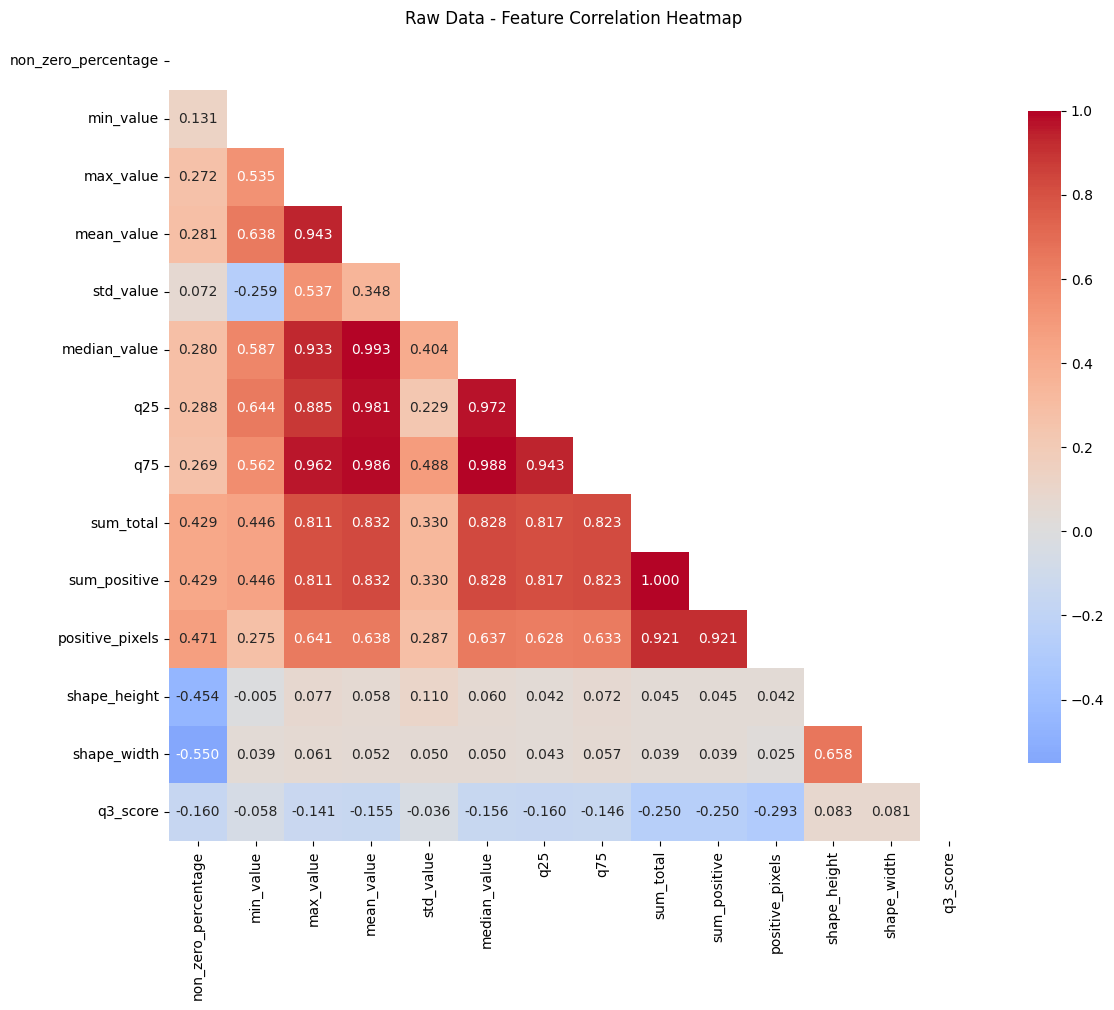
\includegraphics[width=0.9\columnwidth]{plots/corr_vga_q3.png}
    \captionof{figure}{Correlation matrix between q3 impression scores, VGA metrics (mean, std, min, max)}
    \label{fig:corr_vga_q3}
\end{flushleft}

\begin{flushleft}
    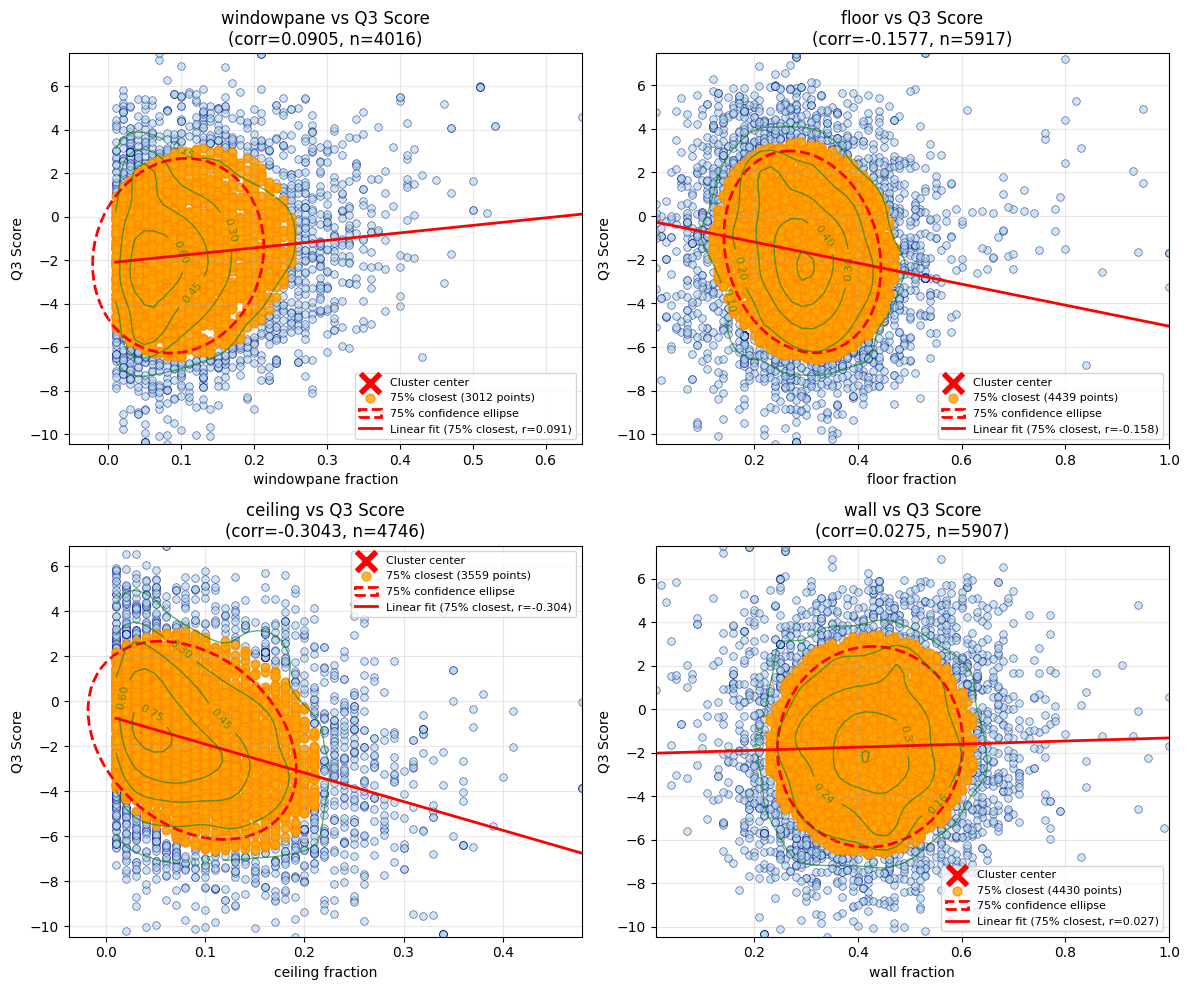
\includegraphics[width=0.9\columnwidth]{plots/inter_q3_cluster.png}
    \captionof{figure}{2D distributions of q3 scores vs. interior semantic segmentation component ratios}
    \label{fig:inter_q3_cluster}
\end{flushleft}

\begin{flushleft}
    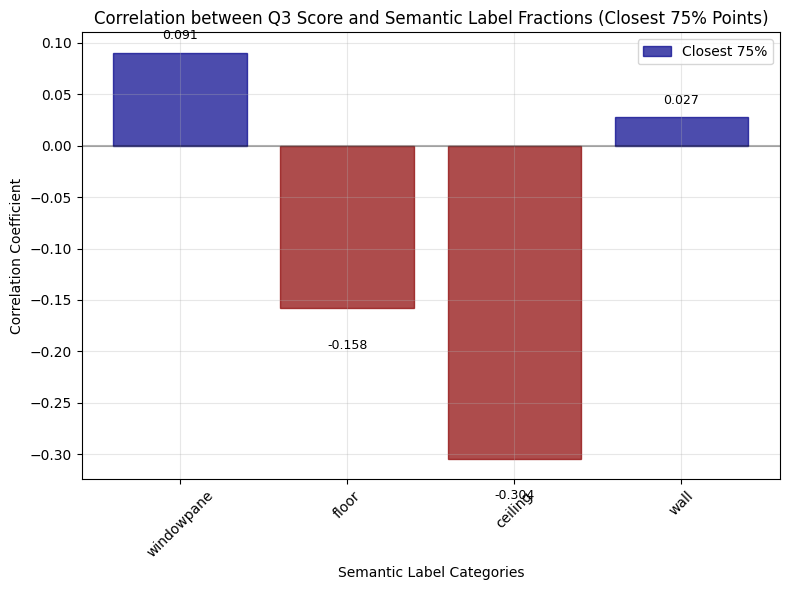
\includegraphics[width=0.9\columnwidth]{plots/corr_inter_q3.png}
    \captionof{figure}{Correlation analysis between q3 scores and semantic segmentation ratios after outlier filtering}
    \label{fig:corr_inter_q3}
\end{flushleft}





% Additionally, Figure \ref{fig:pie_type} shows the distribution of property types in our dataset, 
% providing context for the composition of analyzed rental properties.

% \begin{flushleft}
%     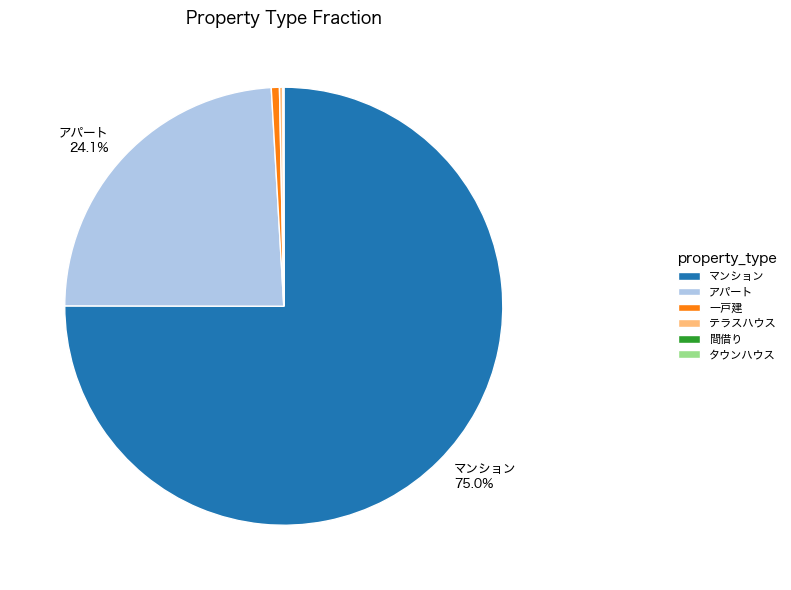
\includegraphics[width=0.7\columnwidth]{plots/pie_type.png}
%     \captionof{figure}{Distribution of property types in the analyzed dataset}
%     \label{fig:pie_type}
% \end{flushleft}

Detailed analysis will be presented in the full thesis.



\section{Conclusion and Future Work}

This research presents a framework for analyzing spatial openness in rental housing through automated madori
interpretation, visibility graph analysis, and interior semantic segmentation. Our methodology quantifies subjective 
spatial qualities using visual data from rental platforms for scalable urban analysis. Key findings reveal weak 
correlations between VGA metrics and user impression scores, with interior segmentation showing that excessive 
floor/ceiling visibility negatively impacts quality perceptions. Limitations include: (1) q3 impression scores 
with potential alignment bias, (2) VGA accuracy depending on segmentation quality, and (3) interior segmentation 
capturing visual elements rather than aesthetic qualities. Future work should improve scoring methodologies, 
segmentation validation, and integrate aesthetic analysis. This open-source framework provides practical tools 
for data-driven spatial quality assessment in real estate and urban planning.

\section{References}

[References would be listed here.]

\end{multicols}

\newpage

\begin{multicols}{2}
\fontsize{11}{13}\selectfont

% Additional content for page 3 would continue here
% This could include detailed methodology descriptions,
% additional results, or extended discussion sections

\end{multicols}

\newpage

\begin{multicols}{2}
\fontsize{11}{13}\selectfont

% Final page content would be placed here
% This might include appendices, additional references,
% or supplementary analysis results

\end{multicols}

\end{document}